\section{Mode 2 - Hand tracking}

\subsection{Mode description}

This mode allows the user to control directly the head of the robot. The principle is simple: the program tracks the finger of the user with the help of the Leap Motion sensor. The position is then scaled to fit in the robot moving area (over the table for instance). A command is issued to order the robot to move to the calculated position. For testing simplicity, the movements are only allowed over two axes, x and y (you cannot go up), but adding a new direction of movement could be done in a matter of minutes.
One important thing one could notice is that there is no delay in the information sent to the robot. This lack of a delay is due to the fact that for this particular part it does not matter if the robot misses a few positions, the movement being executed in a small area.
At the same time the robot is drawing, a window is opened with OpenCV in order to draw on the screen.

The black part in the following Figure \ref{fig:cloudNotCloud} corresponds to the drawing without filtering.

\begin{figure}[H]
	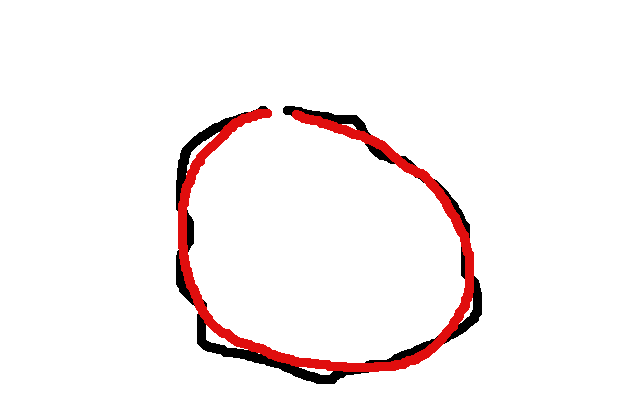
\includegraphics[scale = 0.5]{cloudNotCloud}
	\centering
	\caption{Example of drawing before and after filter applied}
	\label{fig:cloudNotCloud}
\end{figure}

In the Figure \ref{fig:cloudNotCloud} an exemplary output image is shown. It is not the exact set of coordinates that was sent to the robot, but only a tool that helps the user tracking the path of the finger's movement. As it was mentioned before, commands are sent in the real time and some points drawn in the image are missed. Thus, the image made by the robot is a more interpolated and digitized version of an output of the finger tracking displayed on the screen.

\subsection{Filter}

One of the objectives of this project was to make the Leap Motion less sensible to noise. There are many way to do that and many types of existing filters. But as far as our testing went a simple mean filter is more than enough to stabilize the output of the dynamic mode. The mean filter can be set to work on a different number of positions (the $n$ previous ones).
One example of the output of the filter is presented in the Figure \ref{fig:cloudNotCloud} as the red line. As can be seen in the figure, the black line is smoothed and the noise caused by the natural shaking of the operator's hand is reduced.

\begin{figure}[H]
	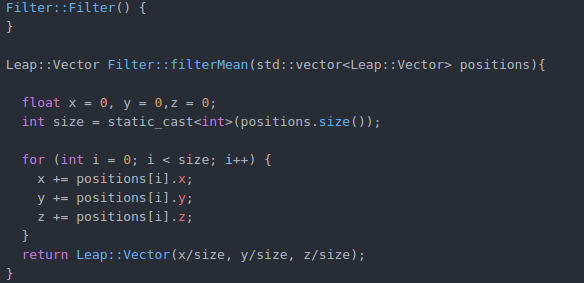
\includegraphics[scale = 0.5]{codeFilter}
	\centering
	\caption{Code of the filter}
	\label{fig:filter}
\end{figure}

The mean filter is easy to implement as seen in the Figure \ref{fig:filter}, but it can also cause some issues. The most important thing in this case is the number of previous positions used. When that size is too small the filter is not working well, because the averaged coordinates are almost the same as that ones given directly from the Leap Motion. On the other hand, a greater number of positions also has one serious drawback - the hand tracking is very slow and the program is not sensitive enough to the finger's movement. After several attempts and combinations the proper number was found and improvements were easy to spot on the screen.
